%v1.8

\documentclass[11pt, mscthesis]{usiinfthesis}
\usepackage[utf8]{inputenc}
\usepackage[english]{babel}
\usepackage{lipsum}
\usepackage{listings}
\usepackage{graphicx}
\usepackage{subfig}
\graphicspath{{./images/}{../images/}}
\DeclareGraphicsExtensions{.png,.pdf}

\newcommand{\vect}[1]{\boldsymbol{#1}}

\lstdefinelanguage{algebra}
{morekeywords={import,sort,constructors,observers,transformers,axioms,if,
else,end},
sensitive=false,
morecomment=[l]{//s},
}
\DeclareUnicodeCharacter{0301}{*************************************}


\usepackage{subfiles}
\usepackage{biblatex}
\addbibresource{biblio.bib}

\title{Using Deep Learning to Identify Technical Debt} %compulsory
\specialization{Major in Artificial Intelligence}%optional
\subtitle{Levereging Self Admitted Technical Debt} %optional 
\author{Simone Giacomelli} %compulsory
\begin{committee}
\advisor{Prof. Dr.}{Gabriele Bavota}{} %compulsory
\coadvisor{Dr.}{Csaba Nagy}{}{} %optional
\end{committee}
\Day{1} %compulsory
\Month{September} %compulsory
\Year{2020} %compulsory, put only the year
\place{Lugano} %compulsory

\dedication{Dedication} %optional
%\openepigraph{Someone said \dots}{Someone} %optional

%\makeindex %optional, also comment out \theindex at the end

\begin{document}

\maketitle %generates the titlepage, this is FIXED

\frontmatter %generates the frontmatter, this is FIXED

\begin{abstract}
Composed of four parts: \\
a: context\\
b: problem\\
c: proposed solution\\
d: results\\
\\
max 400 words.
I will write it once the intro has been approved
\\
\\
\\

\end{abstract}

% \begin{abstract}[Zusammenfassung]
% optional, use only if your external advisor requires it in his/er
% language 
% \\

% \lipsum
% \end{abstract}

\begin{acknowledgements}
Ack 
\end{acknowledgements}

\tableofcontents 
\listoffigures %optional
\listoftables %optional

\mainmatter

%1
\chapter{Introduction}
Technical Debt (TD) is a metaphor between the financial concept and software development.
A TD is contracted when a workaround or shortcut is taken during code implementation.
Choosing an easy and quick solution over a slower and more correct one gives the benefit to save time and deliver the artifact faster. 
\\
The downsides of incurring in TD are many, one of the most intuitive is that further work on the affected parts will be more expensive and time consuming than on clean and healthy code. There are also indirect effects to contemplate: the software could misbehave in the domain it is operating, causing costs and damages as the effect of unexpected output or wrong behavior.
\\
TD do not only appear in software projects but can also be found in many layers of a technology stack: for example, delaying an hardware upgrade or a maintenance can give an immediate benefit of less downtime or financial savings, but an increased cost for future unexpected downtime or failures \cite{allman2012managing}.
\\
Developers or managers can choose to incur in TD because of strict deadline, limited resources available or just plain laziness \cite{hinsen2015technical,allman2012managing}. Cunningham, who coined the technical debt metaphor, writes in "The WyCash portfolio management system" \cite{cunningham1992wycash}: "A little debt speeds development so long as it is paid back promptly with a rewrite". Cunningham implies that one could benefit from a small amount of TD but its should be paid back as soon as possible. 
\\
TD can arise from intentional and unintentional decision, an inexperienced person could contract it without being aware of it \cite{hinsen2015technical}; In both cases it's often done for saving the limited available resources and shortening time-to-market \cite{tom2012consolidated}. For example, startups are highly pressured to quickly test products and ideas in order to save capitals and be faster than competitors.
Besker at al. studied how startups incur in TD, which are the factors, challenges and benefits of intentional acquisition of TD; two of the regulating factors found by the authors are the experience of the developers and the software knowledge of the founders \cite{besker2018embracing}.
\\
In contrast to the beneficial viewpoint of TD, Ron Jeffries argues that the metaphor could be "perhaps too gentle", because it highlights the wise aspect of the choice of contracting a debt; the problem is that people also takes debt unwisely.
Technical debt benefits a software project as long as it is handled before the bigger long term cost is realized \cite{guo2016exploring}.
\\
In order to better analyze and create a tractable model of TD, Alves et al. identifies three variables \cite{martini2018technical}: 


Identified variables (3)
Tracking and managing is important
Few proposed tracking and managing examples

there is a cost paying the debt and there are interest costs when efforts are wasted coping with non optimal code.



Why detecting it is important\\
Tom et al. in their systematic literature review studied, among others, the benefits and drawbacks of incurring in TD \cite{tom2012consolidated}; the part we are now interested in is the drawbacks: 
\\
Increasing costs over time, such as the amount of effort required to deliver a certain amount of functionality 
\\
Work estimation becomes difficult
\\
Developer productivity is negatively impacted 
\\
Becomes increasingly difficult to repay as decisions are affected by existing debt 
\\
Increased risk involved in modifications to the system
\\
Change becomes prohibitively expensive to the point of bankruptcy, and a complete rewrite
and new platform may become necessary
\\
Decreased quality in the end product
\\
\\
Ci sono team che risolvo as-you-go, altri hanno strategie per rilevare, identificare e fixare.
It has been studied that TD [Investigating the Impact of Design Debt on Software Quality]
E' importante rilevare e monitorare i TD perche' questi aumentano il costo di un progetto software, costo dovuto dall'interesse che si deve pagare in relazione al TD.

\newpage



%1.1

\section{Objectives and Results}
Once the context is clear, I will explain the goal of the thesis and summarize the achieved results
The goal of the thesis is to exploit SATD to train a model that can acquire the capacity to distinguish between TD-free code and code affected by TD.
Using the comments in open source projects I will identify class methods noted as SATD. Through the vcs commit history I will identify when this comments disappear; the assumption here is that when the comment is removed from the code the SATD has been fixed. Many cases are excluded to minimize the probability of keeping a false positive, i.e. the SATD is not fixed but the comment is removed. For example, the simplest case excluded is when the code is exactly the same and the only change is the SATD comment removal. Another reason of exclusion is when the code is changed too much; in such case it would not be prudent to keep the sample in the dataset.

The achieved results tell us that it is difficult to predict with high accuracy on methods with big bodies. As the train dataset is limited to shorter and shorter method size, the accuracy grows. 


%1.2
\section{Structure of the Thesis}
A simple bullet list saying "Chapter 2 presents the state of the art, bla... Chapter 3 ..."
\\
\\

\begin{itemize}
  \item Chapter 2 presents the state of the art
  \item Chapter 3 explains how to leverage SATD to train a Deep Learning model to detect TD
  \item Chapter 4 Empirical Study design
  \item Chapter 5 Results discussion
  \item Chapter 6 Threats to validity
  \item Chapter 7 Conclusion
\end{itemize}



%2
\chapter{State of the Art}
The following chapters describe existing approaches to detect different types of technical debt

%2.1

%2.1
\section{Automatic Identification of Software Bugs}
Classification of bug detection tools.\\
The following table needs to be customized\\
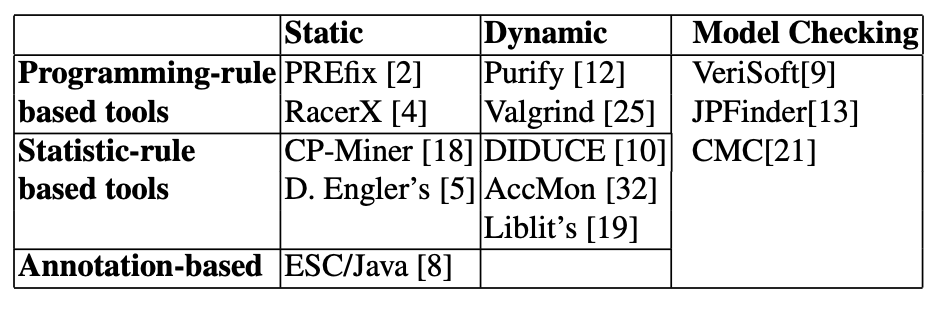
\includegraphics{classification-of-bug-detection-tools.png}
\\
\textbf{PREfix} is a source code analyzer that detects a broad range of errors in C and C++ code \cite{bush2000static}.
Its goal is to detect many runtime issues on real world programs, without dynamic analysis and instrumentation; only the source code text is used. PREfix can detect defects efficiently through a model that abstracts functions and their interactions; the analyzer traces execution paths handling multiple language features: pointers, arrays, structs, bit field operations, control flows statements and so on.
The method used is based on the simulation of individual functions; it uses a virtual machine that simulates the actions of each operator and function call. With the detailed tracking it can report defects information to the user so to easily characterize the detected error.
The tool can be applied both to a complete program source or only a subset. This bottom up approach is particularly useful when the source code is not fully available (e.g. in the case of a thirty part library).
\\
\\
\textbf{RacerX} deals with complex multithread systems. It detects race conditions and deadlock using static analysis \cite{engler2003racerx}.
The tool can infer from the source code the object lock that is assigned to a particular code block. It detects code that is multithreaded and the code that apply dangerous shared access. 
RaceX uses annotations only to mark the code that deals with lock acquisition; this requirement keeps the burden on the user to the minimum to increase ease of adoption. The authors of RaceX report their experiences on the biggest problem about race detection: in large codebase there are massive amounts of unprotected variable access; the key point is to report only those that can actually cause problems. There is emphasis on two aspects. The first is to minimize the impact of reporting false positive in order to avoid the users to discard the use of the tool; to achieve this, RaceX employs specific techniques to lower the impact of analysis mistakes. The second is the speed of the tool: the authors keep the time of execution for the analysis under deep scrutiny; they claim that for a codebase of 1.8 LOC the time required is between 2-14 minutes. The tool has been found capable of finding sever problems in huge projects like Linux, FreeBSD and a large closed source commercial software.
\\
\\

\textbf{Purify}
 is a dynamic  analysis tool for software testing and quality assurance \cite{hastings1992fast}. 
 It instruments the object code files generated from compilers (the software dates back to 1992 and the supported platform is Sun Microsystem's SPARC); the target object files include also third-party libraries. Purify detects multiple errors: memory leaks, access error, reading uninitialized memory. The injected instructions check every read and write memory operations; the slow down of the target is under three times in respect to the non-instrumented execution time. The authors emphasizes: the ease of use in the classic makefile development toolchain and the low overhead that allows the developer to detect bugs early on in the development cycle.
\\
\\
\textbf{Valgrind [25] todo: this is copy\&paste of the website description and wikipedia}
Valgrind is an instrumentation framework for building dynamic analysis tools. There are Valgrind tools that can automatically detect many memory management and threading bugs, and profile your programs in detail. You can also use Valgrind to build new tools.

[wikipedia]
Valgrind is in essence a virtual machine using just-in-time (JIT) compilation techniques, including dynamic recompilation. Nothing from the original program ever gets run directly on the host processor. Instead, Valgrind first translates the program into a temporary, simpler form called Intermediate Representation (IR), which is a processor-neutral, SSA-based form. After the conversion, a tool (see below) is free to do whatever transformations it would like on the IR, before Valgrind translates the IR back into machine code and lets the host processor run it. Valgrind recompiles binary code to run on host and target (or simulated) CPUs of the same architecture. It also includes a GDB stub to allow debugging of the target program as it runs in Valgrind, with "monitor commands" that allow you to query the Valgrind tool for various sorts of information.

A considerable amount of performance is lost in these transformations (and usually, the code the tool inserts); usually, code run with Valgrind and the "none" tool (which does nothing to the IR) runs at 1/4 to 1/5 of the speed of the normal program.
\\
\\
\textbf{CP-Miner [18] todo: this is copy\&paste of the paper abstract}
Copy-pasted code is very common in large software be- cause programmers prefer reusing code via copy-paste in order to reduce programming effort. Recent studies show that copy-paste is prone to introducing bugs and a sig- nificant portion of operating system bugs concentrate in copy-pasted code. Unfortunately, it is challenging to ef- ficiently identify copy-pasted code in large software. Ex- isting copy-paste detection tools are either not scalable to large software, or cannot handle small modifications in copy-pasted code. Furthermore, few tools are available to detect copy-paste related bugs.
In this paper we propose a tool, CP-Miner, that uses data mining techniques to efficiently identify copy-pasted code in large software including operating systems, and detects copy-paste related bugs. Specifically, it takes less than 20 minutes for CP-Miner to identify 190,000 copy- pasted segments in Linux and 150,000 in FreeBSD. More- over, CP-Miner has detected 28 copy-paste related bugs in the latest version of Linux and 23 in FreeBSD. In addition, we analyze some interesting characteristics of copy-paste in Linux and FreeBSD, including the distribution of copy- pasted code across different length, granularity, modules, degrees of modification, and various software versions.
\\
\\
\textbf{D. Engler's [5] todo: this is copy\&paste of the paper abstract}
A major obstacle to finding program errors in a real system is knowing what correctness rules the system must obey. These rules are often undocumented or specified in an ad hoc manner. This paper demonstrates techniques that automatically extract such checking information from the source code itself, rather than the programmer, thereby avoiding the need for a priori knowledge of system rules.The cornerstone of our approach is inferring programmer "beliefs" that we then cross-check for contradictions. Beliefs are facts implied by code: a dereference of a pointer, p, implies a belief that p is non-null, a call to "unlock(1)" implies that 1 was locked, etc. For beliefs we know the programmer must hold, such as the pointer dereference above, we immediately flag contradictions as errors. For beliefs that the programmer may hold, we can assume these beliefs hold and use a statistical analysis to rank the resulting errors from most to least likely. For example, a call to "spin\_lock" followed once by a call to "spin\_unlock" implies that the programmer may have paired these calls by coincidence. If the pairing happens 999 out of 1000 times, though, then it is probably a valid belief and the sole deviation a probable error. The key feature of this approach is that it requires no a priori knowledge of truth: if two beliefs contradict, we know that one is an error without knowing what the correct belief is.Conceptually, our checkers extract beliefs by tailoring rule "templates" to a system --- for example, finding all functions that fit the rule template "a must be paired with b." We have developed six checkers that follow this conceptual framework. They find hundreds of bugs in real systems such as Linux and OpenBSD. From our experience, they give a dramatic reduction in the manual effort needed to check a large system. Compared to our previous work [9], these template checkers find ten to one hundred times more rule instances and derive properties we found impractical to specify manually.
\\
\\
\textbf{DIDUCE [10] todo: this is copy\&paste of the paper abstract}
DIDUCE is a practical and effective tool that aids programmers in detecting complex program errors and identifying their root causes. By instrumenting a program and observing its behavior as it runs, DIDUCE dynamically formulates hypotheses of invariants obeyed by the program. DIDUCE hypothesizes the strictest invariants at the beginning, and gradually relaxes the hypothesis as violations are detected to allow for new behavior. The violations reported help users to catch software bugs as soon as they occur. They also give programmers new visibility into the behavior of the programs such as identifying rare corner cases in the program logic or even locating hidden errors that corrupt the program's results.We implemented the DIDUCE system for Java programs and applied it to four programs of significant size and complexity. DIDUCE succeeded in identifying the root causes of programming errors in each of the programs quickly and automatically. In particular, DIDUCE is effective in isolating a timing-dependent bug in a released JSSE (Java Secure Socket Extension) library, which would have taken an experienced programmer days to find. Our experience suggests that detecting and checking program invariants dynamically is a simple and effective methodology for debugging many different kinds of program errors across a wide variety of application domains.
\\
\\
\textbf{AccMon [32] todo: this is copy\&paste of the paper abstract}

This paper makes two contributions to architectural support for software debugging. First, it proposes a novel statistics-based, on- the-fly bug detection method called PC-based invariant detection. The idea is based on the observation that, in most programs, a given memory location is typically accessed by only a few instructions. Therefore, by capturing the invariant of the set of PCs that nor- mally access a given variable, we can detect accesses by outlier instructions, which are often caused by memory corruption, buffer overflow, stack smashing or other memory-related bugs. Since this method is statistics-based, it can detect bugs that do not violate any programming rules and that, therefore, are likely to be missed by many existing tools. The second contribution is a novel architec- tural extension called the Check Look-aside Buffer (CLB). The CLB uses a Bloom filter to reduce monitoring overheads in the recently- proposed iWatcher architectural framework for software debugging. The CLB significantly reduces the overhead of PC-based invariant debugging.
We demonstrate a PC-based invariant detection tool called Ac- cMon that leverages architectural, run-time system and compiler support. Our experimental results with seven buggy applications and a total of ten bugs, show that AccMon can detect all ten bugs with few false alarms (0 for five applications and 2-8 for two appli- cations) and with low overhead (0.24-2.88 times). Several existing tools evaluated, including Purify, CCured and value-based invariant detection tools, fail to detect some of the bugs. In addition, Purify’s overhead is one order of magnitude higher than AccMon’s. Finally, we show that the CLB is very effective at reducing overhead.
\\
\\
\noindent \textbf{Liblit's [19] todo: this is copy\&paste of the paper abstract}
We propose a low-overhead sampling infrastructure for gath- ering information from the executions experienced by a pro- gram’s user community. Several example applications illus- trate ways to use sampled instrumentation to isolate bugs. Assertion-dense code can be transformed to share the cost of assertions among many users. Lacking assertions, broad guesses can be made about predicates that predict program errors and a process of elimination used to whittle these down to the true bug. Finally, even for non-deterministic bugs such as memory corruption, statistical modeling based on logistic regression allows us to identify program behaviors that are strongly correlated with failure and are therefore likely places to look for the error.
\\
\\
\textbf{ESC/Java [8] todo: this is copy\&paste of the paper abstract}
Software development and maintenance are costly endeavors. The cost can be reduced if more software defects are detected earlier in the development cycle. This paper introduces the Extended Static Checker for Java (ESC/Java), an experimental compile-time program checker that finds common programming errors. The checker is powered by verification-condition generation and automatic theoremproving techniques. It provides programmers with a simple annotation language with which programmer design decisions can be expressed formally. ESC/Java examines the annotated software and warns of inconsistencies between the design decisions recorded in the annotations and the actual code, and also warns of potential runtime errors in the code. This paper gives an overview of the checker architecture and annotation language and describes our experience applying the checker to tens of thousands of lines of Java programs.
\\
\\
\textbf{VeriSoft [9] todo: this is copy\&paste of the paper abstract}
VeriSoft is a tool for systematically exploring the state spaces of systems composed of several concurrent processes executing arbitrary code written in full-fledged programming languages such as C or C++. It can automatically detect coordination problems between concurrent processes. Specifically, VeriSoft searches the state space of the system for deadlocks, livelocks, divergences, and violations of user-specified assertions. An interactive graphical simulator/debugger is also available for following the execution of all the processes of the concurrent system.
\\
https://link.springer.com/chapter/10.1007/3-540-63166-6\_52
\\
\\
\textbf{JPFinder [13] todo: this is copy\&paste of the paper abstract}
Jpf, is a prototype translator from Java to Promela, the modeling language of the Spin model checker [4]. Jpf is a product of a major effort by the Automated Software Engineering group at NASA Ames to make model checking technology part of the software process. Experience has shown that severe bugs can be found in final code using this technique [1], and that automated translation from a programming language to a modeling language like Promela can help reducing the effort required.
Jpf allows a programmer to annotate his Java program with assertions and verify them using the Spin model checker. In addition, deadlocks can be identi- fied. An assertion is written as a call to an assert method defined in a predefined Java class, the Verify class. The argument to the method is a boolean Java expression over the state variables. The Verify class contains additional tem- poral logic methods which allow to state temporal logic properties about static variables. Hence Java itself is used as the specification language. An application of Jpf is described elsewhere in the proceedings [3].
A respectable subset of Java is covered by Jpf, including dynamic object cre- ation, object references as first class citizens, inheritance, exceptions, interrupts, and perhaps most importantly: thread operations. Among major concepts not translated are: packages, method overloading and overriding, method recursion, strings, and floating point numbers. Finally, the class library is not translated
\\
\\
\textbf{CMC [21] todo: this is copy\&paste of the paper abstract}
Many system errors do not emerge unless some intricate sequence of events occurs. In practice, this means that most systems have errors that only trigger after days or weeks of execution. Model checking [4] is an effective way to find such subtle errors. It takes a simplified description of the code and exhaustively tests it on all inputs, using techniques to explore vast state spaces efficiently. Unfortunately, while model checking systems code would be wonderful, it is almost never done in practice: building models is just too hard. It can take significantly more time to write a model than it did to write the code. Furthermore, by checking an abstraction of the code rather than the code itself, it is easy to miss errors.
The paper's first contribution is a new model checker, CMC, which checks C and C++ implementations directly, eliminating the need for a separate abstract description of the system behavior. This has two major advantages: it reduces the effort to use model checking, and it reduces missed errors as well as time-wasting false error reports resulting from inconsistencies between the abstract description and the actual implementation. In addition, changes in the implementation can be checked immediately without updating a high-level description.

The paper's second contribution is demonstrating that CMC works well on real code by applying it to three implementations of the Ad-hoc On-demand Distance Vector (AODV) networking protocol [7]. We found 34 distinct errors (roughly one bug per 328 lines of code), including a bug in the AODV specification itself. Given our experience building systems, it appears that the approach will work well in other contexts, and especially well for other networking protocols.

%2.2
\section{Code Smells and Anti-patterns}
This section explains briefly what code smells and anti-patterns are. The following sections contain the most interesting contribution from the literature on the subject.
\\
\\
An Anti-pattern is a common poor solution to a design problem. It presents itself in object-oriented based systems where a developer applies a solution that is usually ineffective or worse, harmful.
The term stems from its correct and desirable counter part: design pattern.
Design pattern is defined as a reusable solution to a commonly occurring problem within a given context in software design.

Anti-patterns are well known to have negative effects on software projects: they hinder code comprehension, and increase maintenance costs.

A code smell is any aspect of the source code that hint to a deeper problem; in other words they are symptoms of a potential bigger issue. It does not always indicate that a real problem exists but it suggests to look closer and inspect if something more profound is present.

It must be said that neither anti-patterns nor code smells are strictly bugs: in fact, they do not imply incorrect results and they do not stop the program from functioning. Nevertheless, for the risks specified above, automatic detection of code smells and anti-patterns received a lot of attention. 

In the following sections, we will report several contributions from the literature that start to be available in earnest from roughly 1995.

% \textbf{copy\&paste}
% Several techniques have been proposed in the literature to detect code smell instances affecting code components, and all of these take their cue from the suggestions provided by four well-known books: [29], [16], [86], [66].

\subsection{Four inspirational books description}

There are four books that inspired many automatic detection techniques. The first editions of these books span from year 1995 to 1999. 
The following paragraphs describe them briefly.
\\
\\
%smell-book-a
\textbf{Webster} \cite{webster1995pitfalls} Pitfalls of object-oriented development

This book analyzes the cycle of object oriented programming shedding light on its weaknesses and shortcomings. It compares and explains OOP and previous programming techniques. It provides insight and counsel on how to avoid OOP risks.
\\
\\
%smell-book-b
\textbf{Riel} \cite{riel1996object} Object-oriented Design Heuristics

The author provide the reader with metrics to understand the quality of the object-oriented software. The book explains guidelines to help make better decisions on the design of the OO system. 
The sixty recommendations in this book are language-independent and help the reader to evaluate the quality of a software design.
\\
\\
%smell-book-c
\textbf{Fowler} \cite{fowler2018refactoring} Refactoring: improving the design of existing code

The objective of this book is to give practical refactoring strategies to apply on projects so to improve the design of existing systems. It describes many code smells and for each it explains the appropriate actions to take to fix the problem. The first edition dates back to 1999.
\\
\\
%smell-book-d
\textbf{Brown et al.} \cite{brownantipatterns} AntiPatterns: Refactoring Software, Architectures, and Projects in Crisis

The reader finds the detailed description of 40 anti-patterns divided in three categories: managerial, architectural and developmental. 
Each anti-pattern entry is a card with many key aspects, e.g. name, description, root causes, symptoms and an optional anecdotal evidence.
\\
\\
\subsection{Last decade proposed approaches}
Many proposal for design flaws identification have been done in the last decade; many of them have some of their roots in previous mentioned books.
\\
\\
%smell-1
\textbf{Travassos et al.} \cite{travassos1999detecting} Detecting defects in object-oriented designs: using reading techniques to increase software quality

Travassos et al. created a set of techniques to identify manually defects in order to improve software quality. These practices help individuals to read object oriented code and assess, through a predefined taxonomy. The authors conducted an empirical study on these techniques and reported their feasibility.
\\
\\
%smell-2
\textbf{jCOSMO} \cite{van2002java} Java quality assurance by detecting code smells

This paper presents an approach to automate the detection of code smells. The authors assess that code smells are not precise and formal and need human intuition to appreciate them; the outcome of this observation is that a tool to automatically detect code smells needs to be user configurable.
They developed a tool based on these ideas, jCOSMO, that comes already configured to detect two specific code smells (instanceof and typecast). The customization deals with three aspects on code smells: inclusion of new ones, exclusion and fine tuning for more precise definitions.
The users of jCOSMO can benefit of automatic detection and graphical visualization of the results.
\\
\\
%smell-3
\textbf{Simon et al.} \cite{simon2001metrics} Metrics based refactoring

The authors agree that the developer is the last authority with the power to decide where to apply refactoring techniques. One of their contributions is providing them with metrics to support subjective perception regarding code smells. They believe that a key issue is helping developers with tools that support human intuition. 
The authors demonstrate that metrics are effective in finding and pointing to places where code anomalies are detected. These are the presented refactorings: move method, move attribute, extract class and inline class.
\\
\\
%smell-4
\textbf{Marinescu} \cite{marinescu2004detection} Detection strategies: Metrics-based rules for detecting design flaws

Marinescu observed that there are multiple problems using quality metrics to improve software quality. Often the definition of the metrics are imprecise, confusing or incomplete. Another issue is the interpretation of the metrics; they seldom provide a model that help to correctly understand and apply them to a concrete situation. 
Using the metrics in isolation leads to excessive detail and it becomes difficult to use this information to investigate design flaws. In other words, an isolate measure can be helpful to identify the presence of an anomaly but it does not point to the cause; this leaves the developer without a meaningful insight on how to handle the refactoring. The author calls this `bottom-up' approach.
Marinescu proposes a novel method called \emph{detection strategy} to overcome this problem; it's a `top-down' approach that starts from an abstract high level goal and drives the investigation of design trait that conforms to the strategy.
This technique was applied to ten detection strategies and used on industrial case studies; the result of the experiment proved that the method is applicable and usable in practice.
\\
\\
%smell-5
\textbf{Lanza and Marinescu} \cite{lanza2007object} Object-oriented metrics in practice: using software metrics to characterize, evaluate, and improve the design of object-oriented systems

The ideal reader of this book, as defined by the book itself, is a fluent programmer who concretely deals with the maintenance and evolution of a complex large application.
This text uses metrics in a practical way to improve software. It uses them in three phases:
\begin{itemize}
    \item Characterizing the design. The goal is to picture a panorama of the design of the software system. It shows how to use tho metrics-based visualization techniques, \emph{Overview Pyramid} and \emph{Polymetric Views}: Overview Pyramid gives in one shot an overview of the complexity, coupling and inheritance; Polymetric Views shows entities and their relationships supplied with metrics.
    \item Evaluating the design. This phase serves to better understand and assess the design of the application. \emph{Detection strategies} \cite{marinescu2004detection} supply a tool to detect flawed design. \emph{Class Blueprint} is a powerful tool to visualize information about classes, i.e. control-flow and access structure; the goal of this tool is to closely inspect the design flaws detected.
    \item Design disharmonies. There are three categories of disharmonies: Identity, Collaboration and Classification. 
\end{itemize}

The authors, after the identification of disharmonies, propose also insight on how to improve the design through refactoring.
\\
\\
%smell-6
\textbf{Munro} \cite{munro2005product} Product metrics for automatic identification of ``bad smell'' design problems in java source-code

Munro's focus is on automation of bad smell detection in Java source code. The underling motivation of the paper is to enhanced the process for finding places where to apply refactoring. He begins with a precise definition of code smell, building up on the informal definition from Fowler and Beck. The core idea is to analyze the description of the code smell and translate it in measurable attributes that are quantifiable. This process is divided in three phases: informal definition analysis, extract possible quantifiable measures and establishment of rules that are used on the metrics to identify the smells. 
The author applies this process to two specific smells: Lazy Class and Temporary Field. For example, he extracts quality measures as NOM (number of methods), WMC (weighted methods per class), LOC (line of code) and CBO (coupling between objects).
\\
\\
%smell-7
\textbf{Moha et al.} \cite{moha2009decor} DECOR: A method for the specification and detection of code and design smells
\\
The authors split their contributions in three parts. 

The first is DECOR (DEtection and CORrection), it's a method that systematically and formally describes the process to detect code and design smells. It is based on previous work in the field and it leverages the experience and fill the gap of missing features, for example: explicitness on how to specify the detection algorithms, opacity of the technique used, completeness of the analysis on smells description and others. 

The process is defined through five well defined steps: description analysis, specification, processing, detection and validation. The correction part of DECOR, as stated by the authors, is for future work and it is not present in the paper.

The second contribution is DETEX (DETection EXpert); the authors revisit their previous detection technique through the lenses of DECOR and name it DETEX. It uses a DSL to specify smells with high level abstraction and it automatically generates the algorithms for the actual search process. 

The third contribution is an empirical evaluation of DETEX; consistently with the fifth step of DECOR, Moha et al. provides evidence of the application of DETEX on four anti-patterns relating the results in the form of precision and recall. The target of these experiments are eleven open source projects. 
\\
\\
%smell-8
\textbf{Tsantalis and Chatzigeorgiou} \cite{tsantalis2009identification} Identification of move method refactoring opportunities

This paper has a narrow but highly focused contribution: define a process to identify Feature Envy code smells to enable Move Method refactoring.

The authors observe that high coupling and low cohesion are well known indicators of low quality software design; those features are often linked to unwanted outcomes: low maintainability, low productivity and high bug density. 
\\
\\
We can split the proposed process in two parts: identification and ranking.

The identification phase serves to locate candidate methods that could benefit from a move method refactoring. For each method it is evaluated which class could be the destination; this part is driven with distance measures between entities (class, methods and attributes).

The ranking phase serves to avoid overloading the developer with suggestions. This part uses cohesion and coupling as measures to drive the sorting; the metric employed (called Entity Placement) works evaluating the effect of the refactoring without actually modifying the source code.
It is well specified that this is not a fully automated approach because the designer is ultimate responsible on which refactoring should be applied. As one could expect, there are cases where a move method is not a good choice (e.g. moving unit test methods into the target class).

The researchers evaluate their approach with quantitative analysis through the application on two open source-projects. They also track the evolution of the metrics between multiple iteration of refactoring.
They then ask a third party to assess the conceptual validity of the proposed refactoring.
Lastly they also report on the computational cost of their approach.
\\
\\
%smell-9
\textbf{Ligu et al.} \cite{ligu2013identification} Identification of refused bequest code smells

The authors propose a method to identify the Refused Bequest anti-pattern. In synthesis such design smell happens when polymorphism is badly used, for example when a subclass overrides all the superclass methods.
The detection of the smell is achieved with both static and dynamic analyses.
\begin{itemize}
    \item Static analysis is used to identify those class hierarchies that are candidates to potential anomalies.
    \item Dynamic analysis is employed through the exercise of unit testing. The methods of the descendant classes are injected with instructions that intentionally raise an exception; the execution of tests will verify which methods are called or not called, and the result will determine a score towards or away good design. The merge of tests result, from the dynamic analysis, with other structural data generates an output that represents the smell strength.
\end{itemize}
The authors developed an Eclipse plug-in to incorporate the process described above.
\\
\\
\subsection{Code smell detection formulated as an optimization problem}
%smell-10
\textbf{Kessentini et al.} \cite{kessentini2010deviance} Deviance from perfection is a better criterion than closeness to evil when identifying risky code

This paper proposes a novel method in detecting bad smells. The idea that fueled this work is inspired by artificial immune systems; such systems behave in the following way: the more something is detected as different the more it is considered extraneous.
Based on this assumptions, the authors generate a set of detectors that are able to measure various manifestations of anomalies (smells). Thanks to this measurements, they can evaluate how far the system under inspection is from normalcy. 

To be able to create the detectors they need to elect some model to be representative of what normality is; this elected model was taken from the project JHotDraw (by Erich Gamma) that represents, ideally, good design and good programming practices.

The authors report that the results outperform the state of the art and their developed tool is able to detect a good mix of bad smells.
\\
\\
%smell-11
\textbf{Kessentini et al.} \cite{kessentini2014cooperative} A cooperative parallel search-based software engineering approach for code-smells detection

The authors' proposed approach use P-EA (Parallel Evolutionary Algorithms) where multiple algorithms cooperate to find a consensus on the common goal of finding the bad smells. Those algorithms use different adaptations: fitness functions, change operator and solution representations. The cooperation between algorithms happens during the parallel execution in multiple iterations and it is not just a result of one final consensus.

To test the effectiveness of the implementation of the approach, the authors make an empiric comparative evaluation with: random search and two other methods not based on meta heuristics.
The experiment is based on a benchmark of nine large open-source systems; the reported results shows that the approach is better of the state of the art.
\\
\\
%smell-12
\textbf{Boussaa et al.} \cite{boussaa2013competitive} Competitive coevolutionary code-smells detection

The authors propose a novel approach to finding bad smells: they use two populations with their CCEA (Competitive Co-evolutionary Algorithm) search and they employ the use of a code-base sample that contains bad smells. 

The first population goal is to maximize the detection of bad smells thanks to the generation of rules based on quality metrics. 

The second population goal is to maximize the number of synthetic bad smells that the first populations is missing.
\\
\\
The two populations behave similarly to a machine learning GAN framework (Generative Adversarial Network).

The evaluation of the ideas is conducted on four systems through an existing benchmark. The authors reports the statistical analysis: CCEA shows great promise in its performance compared to random and single population approaches.
\\
\\
%smell-13
\textbf{Sahin et al.} \cite{sahin2014code} Code-smell detection as a bilevel problem

The proposed idea and implementation is based on a bilevel optimization. In such formulation there is an outer problem (upper-level) and an inner problem (lower-level).

The upper-level optimization goal is to maximize the detection of bad smells in a sample dataset through the generation of rules based on quality metrics. 

The lower-level maximizes the generation of new artificial bad smell samples that are not detected by the counter part.
\\
\\
The evaluation of the system was performed with 31 runs on nine open source-projects; seven bad smells were detected with an average of more than 86\% in terms of precision and recall.
\\
\\
%different category
\subsection{Non binary classification}
The previous section identified code flaws in a binary class classification (smelly/clean), while the following paragraphs focuses on those analyses that take care of borderline classes.
\\
\\
%smell-14
\textbf{Khomh et al.} \cite{khomh2009bayesian} A bayesian approach for the detection of code and design smells
 
The nature of bad smells contains a measure of uncertainty due to its natural language definition. The authors propose an approach to handle this uncertainty with BBNs (Bayesian Belief Networks). 

Through a systematic process of their own making, the authors convert classic detection rules to a BBNs probabilistic model, using the Blob anti-pattern as their test bench.

They use two open-source projects as targets for the evaluation of the model: GanttProject and Xerces. The authors make a comparison between their model and DECOR and show that it returns the same defective classes plus ordering them by importance.

The last contribution is about exploiting bad smells historical information (in the sense of alternative pre-made dataset) in order to train a machine learning model using Weka; the authors show that this calibration increases the quality of the detection.
\\
\\
%smell-15
\textbf{Oliveto et al.} \cite{oliveto2010numerical} Numerical signatures of antipatterns: An approach based on B-Splines

This paper proposes to overcome two limitations of previous detection technique: the first limitation is the binary classification, there is no in-between or continuous classification of bad smells (e.g. DECOR by Moha et al. \cite{moha2009decor}).
The second limitation is the need of expert knowledge to fuel the detection model (e.g. BBNs by Khom el al. \cite{khomh2009bayesian}).
To overcome these limitations, the authors propose ABS (Antipattern identification using B-Splines). It creates signature of anti-patterns using quality metrics; then it uses the B-spline to create an abstraction of such metrics. This process is applied both to known codes containing bad smells and to unseen unclassified source code; the distance with the B-splines of known anti-patterns measure the similarity to known anti-patterns.
In reference to the second limitation, the authors observe that their technique needs only a dataset but no human intervention and tuning.
\\
\\
%different category
\subsection{Usage of historical data for code smells } 
These two last papers of the section exploit the use of source version control as the basis for their contribution.
\\
\\
%smell-16
\textbf{Ratiu et al.} \cite{rapu2004using} Using history information to improve design flaws detection

The authors propose an idea to make use of historical data on source code to increment performance on the detection of bad smells.
The underling concept is that the evolution of a system can give useful feedback to better determine and analyze the last state of the system.
This paper uses the foundation of \emph{design strategies} (Marinescu \cite{marinescu2004detection}) adding the concept of a system that evolves through time.
The \emph{history} is defined as a sequence of states of the same entity (e.g. system, class and method). The history is used to calculate and evaluate the entity measures \emph{persistence} and \emph{stability}.

The contributions of this paper are: (1) definition of a measure to show how persistent a smell is and how much maintenance effort it absorbed (2) show the improvement in accuracy detecting two class smells (3) describe the valuable information extracted from the history of the anomalies.
\\
\\
%smell-17
\textbf{Palomba et al.} \cite{palomba2014mining} Mining version histories for detecting code smells

This paper shows how to exploit changes on source code to achieve bad smell identification. The history of changes are extracted through the versioning system. 

A novel approach is proposed, called HIST (Historical Information for Smell deTection); it detects five classes of code smells: Divergent Change, Shotgun Surgery, Parallel Inheritance, Feature Envy and Blob.


Using the source history of a project is the only way to detect some bad smells; for example, the Parallel Inheritance smell definition cannot be decoupled from tracking the changes in the code. In other words, the very nature of such smell needs to be able to analyze the changes through time of the system.

There are other kinds of smells that do not strictly need historical data but can benefit from using it; for example, Divergent Change smell and Shotgun Surgery have literature that shows detection approach using last-snapshot information only.

The authors compared the accuracy and recall of HIST with alternative approach and their approach tend to perform better. It is reported that HIST is able to detect smells missed by others (the recall is in range 58\% and 100\%). The previous evaluation was achieved with an empirical study on twenty Java projects; it comprised accuracy and recall calculated against a manually-produced oracle.

A second empirical study represents the closing edge in the loop of the detection process: feedback from the developers of the projects. The goal was to assess at what extent the programmers agreed on the smell detected by HIST: 75\% of the anomalies detected were reported as true problems by the people contacted by the authors (20 developers of 4 projects).
This paper makes available a comprehensive replication package.

%2.3 INSERTED
\section{TD and machine learning}

This section will reference the literature meaningful to this thesis on machine learning and technical debt.
% \\
% (c\&p) Several detection techniques and tools have been proposed in the literature. Recently, the adoption of machine learning techniques to detect bad smells became a trend [20]
\\
\\
%section with antipatterns and smells + ML
%%%%%%%%%%%%%%%%%%%%%%%%%%%%%%%%%%%%%%%%%%

%ml-Khom-27 #cit 208 #powerpoint
%ml-Khom-28 #cit 124
\textbf{Khomh et al.} \cite{khomh2011bdtex} BDTEX: A GQM-based Bayesian approach for the detection of antipatterns

An anti-pattern is defined using natural language; thus, to judge if one is present or not, a human is needed for the decision process.
This work presents an approach to automatically detect anti-pattern while handling the uncertainty inherent to the human-centric process. 

The authors propose BDTEX (Bayesian Detection Expert), an approach to build BBNs (Bayesian Belief Networks) from the definitions of anti-pattern.

First, the authors apply BDTEX on the Blob anti-pattern and describe the advantages of this approach in respect to rule-based techniques.

Second, the method is validated with three anti-patterns: Blob, Functional Decomposition and Spaghetti code. Then the results are compared with those of DECOR \cite{moha2009decor}.
%TODO: FINISH THIS
\\
\\
%ML-fontana-20
%ML-fontana-21
\textbf{Fontana et al. 2013} \cite{fontana2013code} Code smell detection: Towards a machine learning-based approach
\\
\textbf{Fontana et al. 2016} \cite{fontana2016comparing} Comparing and experimenting machine learning techniques for code smell detection

These two papers employ multiple machine learning algorithms for finding code smells. They both use datasets created from the Qualitas Corpus repository \cite{tempero2010qualitas} and manual labelling for creating the ground truth..
The results show an accuracy roughly between 90\% and 95\%. 

Di Nucci et al. \cite{di2018detecting} conducted a study to investigate possible limitations of the two studies above; they found two potential issues that might compromise the effectiveness of the high performance reported. 
First, a single dataset contained smelly samples of only one type. Second, the dataset was unbalanced in respect to the proportion between positive class (smelly) and negative class (non-smelly). 
\\
\\
%ML-Amorim-3
\textbf{Amorim et al.} \cite{amorim2015experience} Experience report: Evaluating the effectiveness of decision trees for detecting code smells

The goal of the authors' is the evaluation of decision tree algorithm on finding code smells. For this study, they use labeled data and code metrics on four Java projects.
They compare their approach with the manual oracle and with the results from three automated finding techniques. 
The comparison shows that the decision tree approach has better performance in most of the cases.

Amorim et al. used the C5.0 algorithm with a 10-fold cross validation and a dataset composed of 7,952 samples. Each sample, which represents an OOP class, has 62 features and 12 binary labels. The features are real numbers depicting source code metrics, for example: line of code, number of parameter and depth of inheritance. The labels represent which code smell affects the class, for example: antisingleton, blob and long parameter list.

The labels related to code smells originated from a work of Khomh et al., \cite{khomh2012exploratory} on the other hand the 62 code metrics are a concatenation between the results obtained by two automated tools (CKJM and POM).

The authors compares the performance of their approach with a rule based technique (using the combined output of four tools) and two machine learning algorithms (SVM and Bayesian Belief Network).
The last experiment reported in the paper, involving the addition of genetic programming, gives an improvement on the performance of the basic approach.
\\
\\
%ML-addon
\textbf{Maldonado et al.} \cite{maldonado2017using} Using natural language processing to automatically detect self-admitted technical debt

This paper shows an approach to automatically detect design and requirement self-admitted technical debt using natural language processing (NLP). 

The experiments use ten Java open-source projects as test bench; the results display a remarkable improvement of performance in respect to the state of the art.
The study exposes the words that best correlates to the studied SATD (design and requirement self-admitted technical debt). 
It is reported that the model behaves very well even using only a fraction (5-23\%) of the training dataset.

The first author of this paper manually classified 29,473 comments extracted from six open-source Java projects. This number was much greater before an automatic filtering using five heuristics: the manual cleaning process is similar to the work from the same authors  \cite{maldonado2015detecting} with an additional filter (removal of comments created by IDEs).
The joining of the newly create dataset with the one from previous work, yields a total number of 62,566 manually classified comments, spanning ten open-source Java systems. These are the SATD classes found: design, defect, documentation, requirement and test debt. 

The classification model employed is the Stanford Classifier which is provided by the The Stanford Natural Language Processing Group \cite{manning2003optimization}; it is a Java software that implements a maximum entropy classifier. It is roughly equivalent to a multi-class logistic regression model.

The training was conducted only on the ordinary comments (i.e. the non-SATD), design and requirement SATD, thus on 61,664 samples.
The results were compared with two baseline with related performance improvement: 
\begin{itemize}
    \item 7.6 and 19.1 times better for design and requirement SATD, respectively compared to a random baseline
    \item 2.3 and 6 times better for design and requirement SATD, respectively compared to comment pattern matching baseline
\end{itemize}

The authors mention which are the characteristics of the vocabulary used by the programmers that strongly indicates SATD (i.e. `hack', `workaround', `yuck!' for design SATD and `todo', `needed', `implementation' for requirement SATD).
\\
\\
\textbf{Ren et al.} \cite{ren2019neural} Neural network-based detection of self-admitted technical debt: from performance to explainability

This study propose a CNN-based approach applied to the identification of SATD. The authors provide the model that includes a method to explain its predictions; the result shows that humans largely agree with the key phrases extracted by the model to explain itself.

It is observed that classic text-mining approaches have limitations in respect to the following measures: performance, generalizability and adaptability. The method described in the paper want to address these issues.

This work documents which are the SATD aspects that influence the above mentioned measures: variant term frequency, project uniqueness, variable length, semantic variation and imbalanced data.

The experiment is conducted on 10 open-source projects with 62,566 code comments.

It is known that the average of SATD over the total number of comments is very low (e.g. between 0.2-2.6\% with average 0.3\%, Bavota and Russo \cite{bavota2016large}; between 3.2-16.8\% with average 7.42\%, Maldonado and Shihab \cite{maldonado2015detecting}; at class level between 0.4-3.33\%, Potdar and Shihab \cite{potdar2014exploratory}). 
Ren et al. reports their SATD concentration to be between 0.41-5.57\% with average 1.86\%; to deal with this unbalanced dataset, they employ a weighted cross-entropy loss and compare the results with the normal loss: the benefit yields an average improvement of 6.22\% on F1-score.
The experiments on tuning reveal which hyper-parameter are the most influential: size of word embedding, number of filter and combination of window size.
The authors conclude that their method improve on explainability and deployability. The first is proven with the high agreement between the SATD summary by the model and humans. The second is explained with a cross-project experiment: the model can be fine-tuned (i.e. transfer learning) with little data and the result proves that it is a highly effective approach.
\\
\\
\textbf{Maipradit et al.} \cite{maipradit2020automated} Automated Identification of On-hold Self-admitted Technical Debt

On-hold SATD are those SATD that can be removed only after a condition is met; in other words, there is an external factor that needs to be waited for before proceeding to remove the TD (e.g. a bug in an issue tracker). 

The authors propose a system to detect on-hold SATD based on regular expression and machine learning; the empirical experiment shows that 8\% of the comments referring to issues are on-hold SATD. The dataset was created from ten open-source projects yielding 133 on-hold satd on a total of 1,530 comments containing issue references.
The classifier developed has an average F1-score of 0.73\% and an average AUC of 0.97\%. 

To evaluate the results, Maipradit et al. collected feedback from the projects' developer about the detected on-hold SATD: there was agreement that they should be fixed or removed.
\\
\\
%ML-Cruz
\textbf{Cruz et al.} \cite{cruz2020detecting} Detecting bad smells with machine learning algorithms: an empirical study

This paper adds empirical evidence on machine learning behavior performing automatic detection of bad smells.

The authors use the Qualitas Corpus \cite{tempero2010qualitas} and extract 20 projects as test bench for this work; they focus the research on four bad smells using seven ML techniques.
It is observed that Gradient Boosting Machine and Random Forest achieved good performance with two bad smells out of four; God Class with F1-score of 0.86 and Refused Parent Bequest of 0.67.

Another contribution is the application of SHAP (SHapley Additive exPlanations, a approach to explain the output of any machine learning) \cite{NIPS2017_7062}. The authors provide an insight on which are the features that are most meaningful for the prediction. 

Cruz et al. created a new datasets to assure quality and perform comparison on an unbalanced dataset (CSV are available for download).
There are four datasets, one for every bad smell, two at class level (God Class, Refused Parent Bequest) and two at method level (Long Method and Feature Envy). Every class has 17 metrics (e.g. Coupling Between Objects and Depth of Inheritance Tree) and every method has 12 metrics (e.g. Lines of Code and Quantity of Loops).
These features are calculated with two tools, VizzMaintenance for the class metrics and CKMetrics for the method metrics.

The ground truth of bad smells was created using five tools: PMD, JDeodorant, JSpirit, DECOR and Organic. The decision if the subject was positive or not was taken by consensus between tools. The authors kept only those smells that could be detected at least by three of the tools; agreement by two of the detectors made a positive case.
The seven algorithms used are: Naive Bayes, Logistic Regression, Multilayer Perceptron, Decision Tree, K-Nearest Neighbors, Random Forest and Gradient Boosting Machine.
\\
\\
\textbf{Wang et al.} \cite{wang2020detecting} Detecting and Explaining Self-Admitted Technical Debts with Attention-based Neural Networks

This paper propose HATD, an attention-based deep learning model, capable of detecting and explaining SATDs. The authors detail which are the important aspects of SATD that need to be analyzed and taken care to successfully implement their proposal. HATD outperforms the state-of-the-art SATD detectors, provides insightful feedback to achieve explainability and is effective when used in real-world projects.

The proposed model is composed by the following parts:
\begin{itemize}
    \item ELMo algorithm for word embedding. In opposition to static word embedding techniques ELMo can deal with polysemy.
    \item Single-head Attention Encoder (SAE). This is used for the explainability of the model.
    \item Multi-head Attention Encoder (MAE). This serves to better encode the current word considering the positional information of the other words in the comment.
    \item A fully connected layer with a weighted cross-entropy loss. This part is feeded with both SAE and MAE output. 
\end{itemize}

The training dataset employed is provided by Maldonado et al. \cite{maldonado2017using}; it was created on ten open-source Java projects and it is known to be imbalanced; to counter this issue, the authors of this paper, introduce a weighted cross entropy loss. 

The initial evaluation of the model is done within- and cross-project.

The within-project evaluation is performed with a 10-fold cross-validation using all ten project.

The cross-project evaluation is implemented using nine projects to train the model and using the remaining project as test set.


The authors asses the capability of HATD to adapt to real-world projects; they select ten additional popular projects from Github. These are written not only in Java but also in Python and Javascript. 

The total number of comments, for these ten projects, are 38,280; HATD detects 543 SATDs, which is 1.33\% of the total. The average concentration of the ten Java projects by Maldonato et al. is, on average 6.57\%.
To check the quality of the predictions, the authors randomly select 100 comments (50 SATD and 50 non-SATD); then they engage five programmers and ask them to classify those comments. The result shows an accuracy of 83\% against the human oracles.
\\
\\
\textbf{Rantala et al.} \cite{rantala2020prevalence} Prevalence, Contents and Automatic Detection of KL-SATD

This paper defines KL-SATD to be Keyword-Labeled self-admitted technical debt. It is a subset of SATDs, i.e. those SATDs that contain specific words that indicates the presence of technical debt admission. The authors focus on four specific keywords: TODO, FIXME, HACK and XXX. The goal is to exploit the information assets contained in KL-SATDs and detect those SATDs that are not KL-SATDs.
\\
\\
The dataset used is provided by Lenarduzzi et al. and includes 33 Java projects \cite{lenarduzzi2019technical}. After pre-processing, the experiment has access to 507,254 comments. One of the first reported finding is the average and median KL-SATD concentration per repository: 2.29\% and 1.52\%, respectively.

The paper highlight the difference in vocabulary used by KL-SATDs and non KL-SATDs; through a word cloud the authors show which are the most common words used (after keywords removal for the KL-SATDs).

A logistic regression classifier is trained to recognize the two above mentioned classes. The 10-fold cross validation has an AUC of 0.88. 


A new dataset is created, formed only by the non KL-SATD comments. Then, the  classifier is executed to make a prediction using this filtered dataset. The authors are interested in those instances labeled as KL-SATD with a confidence over 70\%: these do not contains keywords but could be SATD. To verify this assumption and check if the classifier has learned to spot SATD, two of the authors randomly selected 100 comments and labeled them manually. Using the results, it is estimated that 2/3 of the instances may contain technical debt.









%2.4 -shift down, was 2.3
\section{Technical Debt and Self-Admitted Technical Debt} % proposal for a new title "Technical Debt and Self-Admitted Technical Debt

This section briefly describe the relevant literature to this thesis on the two topic of \emph{technical debt} and later on more specifically on \emph{self-admitted technical debt}.
\\
\\
\subsection{Technical debt literature}
\\
\\
%satd-2
\textbf{Guo et al.} \cite{guo2011tracking} Tracking technical debt - An exploratory case study

This paper aims to highlight and make evident the effect of technical debt on the cost and management of a software project. Through the tracking of a single delayed task in a real project, the authors analyze the consequences of such technical debt. They created a framework for the explicit management of TD and then applied it, with a simulation, to the real scenario under scrutiny.
The objective of this study is:
\begin{itemize}
    \item determine technical debt effects on the project and evaluate their impact
    \item after the application of the simulation, determine if the provided framework gave real gain and uncovered benefits.
\end{itemize}
The results of this simulation made a clear statement that careful planning and analysis of TD is of high importance: in retrospect the cost of the delayed task almost tripled the cost for the project.
\\
\\
%satd-3
\textbf{Klinger et al.} \cite{klinger2011enterprise} An enterprise perspective on technical debt

This short but meaningful study see the design of an interview to four IBM technical architect. One of the authors' goal was to broaden the view on TD from the perspective of a single developer to the perspective of an enterprise.

Starting from the premise that TD can be leveraged as a financial asset (i.e. incur in TD today to gain competitive advantage and repay tomorrow) the study and the interviews are structured to assess how an enterprise handle TD; these are the standpoints:
\begin{itemize}
    \item How decisions to acquire TD are conducted.
    \item What is the leverage gained contracting TD.
\end{itemize}
The following are some of the findings:
\begin{itemize}
    \item Two are the different sources of unintentional contraction of TD: from non-technical stakeholders (e.g. fixing a stringent release date at the expense of software quality) and from external forces (e.g. changes in the market and acquisitions).
    \item The process of acquiring TD was informal. The decision had no written records or written analysis on the impact, effects and expectations of such choice.
    \item A scarcity of knowledge and awareness on the consequences of taking on TD, insufficient channels of communication and lack of a common vocabulary to express contracted costs. 
\end{itemize}
\\
\\
%satd-4
\textbf{Kruchten et al.} \cite{kruchten2012technical} Technical debt: From metaphor to theory and practice

This article expands the original metaphor of technical debt by Cunningham \cite{cunningham1992wycash} in search of a better definition that enables reasoning on a variety of technical debt.
The authors want to lay a theoretical foundation so to be better prepared to take on the challenge of dealing with TD. These are the main points covered by this work:
\begin{itemize}
    \item TD Landscape. It's a possible organization of the many aspects of software improvement. It divides between visible elements (e.g. new features and defects) and mostly invisible (e.g. architecture and code). The idea is that TD is limited to the invisible part
    \item Tackling of TD. The authors reason about the root causes of TD in relation to quality and maintainability issues (so, not directly related to time pressure, e.g. carelessness, lack of education and poor processes) and describe which steps can effectively handle TD (e.g. awareness, explicit management, understand what tools can and cannot do, nurture architecture, documentation)
    \item Unified theory. It is observed that the challenge is making the right sequence of changes to improve the software; in respect to this, perhaps the financial and economic models could be the underling layer to the TD landscape (i.e. expressing all the changes in relation to their cost and value over time).
\end{itemize}
\\
\\
%satd-5
\textbf{Lim et al.} \cite{lim2012balancing} Technical debt: towards a crisper definition report on the 4th international workshop on managing technical debt
 
Lim et al. conducted an interview study on 35 practitioners aimed to define the perceived characteristics of technical debt and in what context TD was encountered. What emerged is most of the teams know well TD and it is an unavoidable necessity in the business reality. Because its certainty, one key factor is active management: recognition, tracking, analysis, cogent decisions and prevention of worst consequences.
 
The participants were queried with both specific and open questions. Aside of general demographic questions, they were asked to describe an example of TD alongside its properties, causes, effects and benefits. 
The answer pointed to a different root cause than sloppy programming and poor discipline. Most of the testimony acknowledged that TD was acquired through an intentional decision; some of those decisions were the results of short-term thinking, yielding to the pressure of the moment.
The negative effects of TD were perceived as long term consequences (e.g. the fear to change code expecting to break other parts of the system). 
In some cases, it was clear that the benefits were far repaid, in others it was not clear if the balance was positive.
The respondents provided many examples of situations that described the crucible for TD (e.g. contracts with stringent deadline, exploiting market opportunity windows). 
\\
The interviewees reported some of their strategies to handle TD:
\begin{itemize}
    \item Do nothing. In those parts where low maintenance is required, it's safer to leave things as they are.
    \item Establish a policy to allocate development resource to fix TD (5 to 10 percent on total resources).
    \item Communication and open dialog about TD between all parties involved (technical, non-technical stakeholders and customers).
    \item Make TD explicit and visible to all the developers (e.g. through audits) and keep track of the discoveries.
\end{itemize}
%satd-6 - SKIP it's a workshop 
% \textbf{Kruchten et al. [24]}
% Kruchten et al. [24] reported their understanding of the technical debt in industry as the result of a four year interaction with practitioners.
% \\
% \\
%satd-7
\textbf{Zazworka et al.} \cite{zazworka2013case} A case study on effectively identifying technical debt
% high valuable information left over that can potentially be added

This paper conducted a study to compare manual and automatic technical debt detection. 

The manual detection was implemented through a questionnaire undertaken by five developers in the same team. The automatic detection was performed using three stable and established tools. 

All questionnaire participants reported different debt (except in on case) so there is almost no consensus in the human component, on the other hand, the results show a good overlap between manual and automatic detection regarding defect debt. Human intervention is still needed for the other types of debt: documentation, design, testing and usability debt; they were, for the most part, unrecognized by automatic tool.
\\
\\
%satd-8
\textbf{Spinola et al.} \cite{spinola2013investigating} Investigating technical debt folklore: Shedding some light on technical debt opinion

The goal of this paper is to provide some guidance on new research questions about TD. Exploiting the folklore extracted from grey literature, the authors gather 14 statements on technical debt; then they proceeded to survey 37 practitioner asking their level of agreement/disagreement on those statements. The most agreed upon was the following: "If technical debt is not managed effectively, maintenance costs will increase at a rate that will eventually outrun the value it delivers to customers".

The underling observation of this paper is that common belief, traditional stories and customs (i.e. folklore) can help the discovery of interesting topics; then, the agreement (i.e. the interview results) of knowledgeable people on those concepts could give a measure of value and worthiness and guide possible future research.
\\
\\
%satd-10
\textbf{Alves et al.} \cite{alves2014towards} Towards an ontology of terms on technical debt

Alves et al. proposed an ontology of terms on technical debt. They developed a \emph{lightweight domain ontology}, designed the quality criteria, conducted a systematic literature mapping and finally submitted the result to a specialist for an evaluation.
\\
The following are the contributions of this work:
\begin{itemize}
    \item The collection and gathering of information that was spread out
    \item The organization of a common vocabulary for the technical debt field 
\end{itemize}
This paper, that describe a common knowledge ground, wants to help researchers and practitioners evolving the Technical Debt Landscape \cite{izurieta2012organizing}.
The first contribution is the organization of 13 types of TD: architecture, build, code, defect, design, documentation, infrastructure, people, process, requirement, service, test automation and test debt.
The second contribution consists in the organization of indicators themselves; these indicators were used to support identification of the TD.
\\
\\
%--------------------------------------------------------------------------------
\subsection{Self-Admitted Technical debt literature}
%satd-1
\textbf{Storey et al.} \cite{storey2008todo} TODO or to bug: Exploring How Task Annotations Play a Role in the Work Practices of Software Developers

This empirical study has the goal to shed light on how the developers behave on personal and team tasks, in respect to source code annotations (i.e. comments).
The authors analyze the relations that annotations have with common used tools like, e.g. wikis, issue and bug trackers. In order to do so, they gathered and combined data coming from a mix of methods, divided in these phases:
\begin{itemize}
    \item Phase 1. Conduction of a survey targeting users of Eclipse IDE. The topic was about annotations: if they did write them, which types and the use of them.
    \item Phase 2. Contextual interviews with developers on three open source projects. Then, augmentation of the answer from the interview with direct analysis on many versions of the source code, related to the annotation in question.
\end{itemize}

The conclusion reports how these finding can be useful to improve tooling and software process.
\\
\\%satd-9
\textbf{Potdar and Shihab} \cite{potdar2014exploratory} An exploratory study on self-admitted technical debt

The authors conducted an empirical study on four open-source projects, focusing on three main research questions reported in the following summary:
\begin{itemize}
    \item Finding the concentration of SATD in the projects
    \item Discovering the reasons for introducing the SATD
    \item Calculating the percentage of SATD removal after its introduction
\end{itemize}

The first contribution is the definition of 62 comment patterns that indicates the presence of a SATD (\emph{e.g. fixme, todo, fix this crap, etc.}); this list of patterns was refined through manually reading 101762 code comments mined from five large open-source projects. 
Using those patterns, they found that between 2.4\% and 31\% of the files contained SATD. Another interesting finding is that experienced practitioners are the most likely to introduce SATD. On the other hand, a counter-intuitive discovery is that the amount of SATD has correlation with neither complexity nor time pressure. The removal ratio was found to be roughly between 0.26 and 0.63.
\\
\\
%satd-9-diff-repl
\textbf{Bavota and Russo} \cite{bavota2016large} A large-scale empirical study on self-admitted technical debt

This study is a differentiated replication of the work by Potdar and Shihab. It is based on the mining of a large source code corpus: 159 software projects that accounted for 600K commits and 2 billion of comments. 
\\
These are the main findings:
\begin{itemize}
\item Diffusion: 51 SATD instances on average per project, that constitutes 0.3\% of the comments.
\item Types: code debt (30\%), defect and requirement debt (20\%) and design debt (13\%).
\item Quality: no correlation is found between the number of SATD and code file internal quality.
\item Evolution
\begin{itemize}
\item Growth: during the history of the project, on average, only 57\% of the introduced SATD are fixed; thus the number of total instances increase over time.
\item Persistence:  those SATD that are fixed (57\%) show a remarkable survivability; they stays in the system, on average, for over 1000 commits.
\item Removal: 63\% of SATD are removed from the same developer that introduced them in the first place; the rest of the time a different and more experienced developer fixes the SATD.
\end{itemize}
\end{itemize}



%satd-11
\textbf{Maldonado and Shihab} \cite{maldonado2015detecting} Detecting and quantifying different types of self-admitted technical debt

The contribution of this paper is the classification of SATD types in four open source projects. The authors manually classified 33093 comments; these are the findings with the range of presence across projects: design debt (42\% - 84\%), requirement debt (5\% - 45\%), defect debt (4\% - 9\%), test debt (0\% - 7\%) and finally documentation debt (0\% - 5\%).

The projects were chosen in the Java realm in different domains with well commented sources: Apache Ant, Apache JMeter, ArgoUml, Columba and JFreeChart. 
Using JDeodorant as comments extractor, the authors gathered more than 166K comments. This number decreased to roughly 33K thanks to processing and filtering of those comments with low likelihood of being SATD. Such operation was conducted through four simple heuristics that targeted the following cases: license comments (removal), commented source code (removal), javadoc (removal), multi line comments instead of block comments (joining). 

The classification process made evident that one SATD can belong to multiple categories (e.g. a design debt can also be a defect debt at the same time). For the sake of clarity this paper will associate only one SATD label to the comment; in case of ambiguity between multiple types, the more meaningful one was chosen. 

The set of possible SATD classes was taken from Alves et al. \cite{alves2014towards} paper. It is observed that not all 13 original TD classes are found in the selected open source projects; Maldonado and Shihab argues that some of the technical debt are not likely to be reported in written comments (e.g. people and infrastructure debt).
The authors report that the personal bias and subjectivity can be a threat to internal validity: the manual classification was executed by only one person (the first author). Other factors on internal validity: quantity and quality of comments could be affected by biased filtering.
About external validity, the authors consider the domain of the projects: it is diverse but all of them are open source Java projects; thus,  the results may not generalize to other languages or market segments.
% This work is closely related to our RQ1, where we man- ually classified the type of technical debt reported in a statistically significant sample of 366 comments. The main differences between our study and the work by Maldonado and Shihab are the scale of the study and the procedure adopted to classify the technical debt instances. Maldon- ado and Shihab analysed a much larger set of comments reporting SATD (33K against 366); However, only one of the authors classified the debt types on the basis of his personal opinion. In our study, we adopted an open coding procedure performed by the two authors to classify the analysed instances and reduce the subjectivity bias. Also, we further refined the technical debt categories defined by Alves et al. [2] as a result of the open coding procedure.
\\
\\
%satd-12
\textbf{Wehaibi et al.} \cite{wehaibi2016examining} Examining the impact of self-admitted technical debt on software quality

This empirical study on five open source projects wants to explore the relation between self-admitted technical debt and defects in source code. It was discovered that that there is an increase of defects after the introduction of SATD. It's also clear that introducing a SATD makes the development on the related code much harder.
\\
\\


%2.4
\section{Summing Up (WAS 2.4)}
Here I explain why what I did is different
\section{Summing Up}

There exist many approaches to detect self-admitted technical debt and technical debt in general. However, to the best of our knowledge, there is no study that leverages the SATD annotations to learn a model that automatically detects technical debt using no meta-information except the bare source code.
In this work we create a dataset of method body pairs (affected with SATD and the fixed counterpart) and train a deep learning model that detects the presence or absence of technical debt in an unseen source code snippet. The study aims to investigate how much the model is able to learn and the correlation of the confidence level on the prediction outcome. Then we analyze where and why it succeeds or fail the prediction.



%3
\chapter{Using Deep Learning to Detect Technical Debt}

Here I describe the approach. 

I'm going to start from a short overview, then I go into details

%3.1
\section{Mining SATD Instances and their Fixes}
\lipsum[1-1]

%3.2 
\section{The Deep Learning Model}

%3.3
\section{Hyperparameter Tuning}
\lipsum[1-1]

%4
\chapter{Empirical Study Design}

I'm going to start with a short description  about the goal/research questions

%4.1
\section{Context Selection}
I'll explain the dataset used for the evaluation
\lipsum[1-1]

%4.2 
\section{Data Collection and Analysis}
How I compute the results


%4.3
\section{Replication Package}
A link to a repo with all data and code




%5
\chapter{Results Discussion}

\dots results discussion \dots 

%5.1
\section{Quantitative Results}
Report precision/recall for different confidence thresholds
\lipsum[1-1]

%5.2 
\section{Qualitative Results}
Discuss interesting cases in which your approach succeeds/fails



%6
\chapter{Threats to Validity}

\dots Discussion on the limitations of my study \dots 


%7
\chapter{Conclusion}

\dots conclusion \dots 

%%%%%%% commented appendix
% \appendix %optional, use only if you have an appendix
% \chapter{Some retarded material}
% \section{It's over\dots}
% \lipsum 

\nocite{*}
\backmatter

%%%%%%% commented glossary
%\chapter{Glossary} %optional

%\bibliographystyle{alpha}
%\bibliographystyle{dcu}
%\bibliographystyle{plainnat}
%\bibliography{biblio}



\printbibliography
%\cleardoublepage
%\theindex %optional, use only if you have an index, must use
%\makeindex in the preamble
\end{document}